\chapter*{2023年\textsf{HDU}「大学物理1s」期中试题解答}

\begin{minipage}{0.32\textwidth}
    \textbf{开课学院}：理学院
      
    \textbf{课程编码}：A071508s
\end{minipage}
\hfill
\begin{minipage}{0.32\textwidth}
    \textbf{解析制作}：\textsc{Meiu Hsia}

    \textbf{\,\hologo{TeX}~排版}：\textsc{Meiu Hsia}
\end{minipage}
\hfill
\begin{minipage}{0.15\textwidth}
    \centering
    \begin{tikzpicture}
        \node [inner sep=0] at (0,0) {
            \qrcode[height=3em,version=4]{https://qm.qq.com/q/mgD30uPiSs}};
        \fill [color=white,rounded corners=(sqrt(2)+2)/11*1em] (-.5em,-.5em) rectangle (.5em,.5em);
        \node [inner sep=0] at (0,0) {\color{MidnightBlue}\scriptsize\faIcon{qq}};
    \end{tikzpicture}

    \scriptsize\href{https://qm.qq.com/q/mgD30uPiSs}{\itshape 未央物理营}
\end{minipage}
\hfill
\begin{minipage}{0.15\textwidth}
    \centering
    \begin{tikzpicture}
        \node [inner sep=0] at (0,0) {
            \qrcode[height=3em,version=4]{http://weixin.qq.com/r/DBIABcHEqgnWKIVmb0eI}};
            \fill [color=white,rounded corners=(sqrt(2)+2)/11*1em] (-.5em,-.5em) rectangle (.5em,.5em);
        \node [inner sep=0] at (0,0) {\color{DarkGreen}\scriptsize\faIcon{weixin}};
    \end{tikzpicture}

    \scriptsize\href{http://weixin.qq.com/r/DBIABcHEqgnWKIVmb0eI}{\itshape 未央学社}
\end{minipage}

\section{Calculate Standard (70 points in all)}

\begin{problem} % {速度，位移}
    A net force with the form $F_x=-4.00+6.00t$ (in SI) is acting on a particle with mass $m=2.00$ (in SI).
    \begin{enumerate}
        \item Find the initial velocity $v_{x_0}$ such that the particle will have the same $x$ coordinate at $t=\qty{2.00}\s$ as it had at $t=\qty{0.00}\s$.
        \item What will be the velocity at $t=\qty{2.00}\s$?
    \end{enumerate}
\end{problem}
\solute{10}
\begin{solution}\leavevmode
    \begin{enumerate}
        \item 质点的加速度$a=F/m=-2+3t$ (SI)，积分得质点在任意时刻$t$的速度大小为
        \[v_x=v_{x_0}+\int_0^t(-2+3t')\d t'=v_{x_0}-2t+\frac32t^2\ \text{(SI)}\]
        再次积分得质点在任意时刻的位置为
        \[x=x_0+\int_0^t{\ab(v_{x_0}-2t'+\frac32t'^2)}\d t'=x_0+v_{x_0}t-t^2+\frac12t^3\ \text{(SI)}\]
        由题意$x(0)=x(2)$得$v_{x_0}=0$ (SI).
        \item $v(2)=v_{x_0}-2\times 2+\frac32\times 2^2=2$ (SI).
    \end{enumerate}
\end{solution}

\begin{paracol}{2}
    \begin{problem} % {转动惯量}
        A thin rod with length $L$ and mass $M$ has density that increase linearly with distance $x$ from the one end, $\rho=\alpha x$, where $\alpha$ is a positive constant. Find the moment of inertia of the rod about an axis through that end of the rod in terms of $L$ and $M$. Is your answer greater or smaller than the moment of inertia of a rod of the same mass and length but of uniform density?
        \switchcolumn\vspace*{\fill}\centering
        \begin{tikzpicture}
            \draw [->] (0,-1) -- (0,1.25);
            \draw [->] (-.2,0) -- (3,0);
            \filldraw [fill=white] (0,.2) rectangle (2.5,-.2);
            \filldraw [semithick,fill=darkgray,opacity=.5] (1.6,.2) rectangle (1.75,-.2);
            \length{(0,-.5)}{(1.675,-.5)}{$x$}{(.5,0)};
            \draw [->] ({.5*sin(15)},{1.25+.2*cos(15)}) arc (75:-255:.5 and .2);
        \end{tikzpicture}\vspace*{\fill}
    \end{problem}
\end{paracol}
\solute{10}
\begin{solution}\leavevmode
    \begin{itemize}
        \item 细棒的质量为$M=\int_0^L{\alpha x\d x}=L^2\alpha/2$，由此得$L^2\alpha=2M$.
        \item $x\sim x+\d x$的微元对转轴的转动惯量为$\d I=x^2\cdot\alpha x\d x$. 对其积分得细棒绕一端旋转的转动惯量$I=\int_0^L\d I=L^4\alpha/4\xlongequal{L^2\alpha=2M}ML^2/2$.
        \item 质地均匀的细棒绕一端旋转的转动惯量$I'=ML^2/3$，该细棒比质地均匀的转动惯量略大.
    \end{itemize}
\end{solution}

\begin{problem} % {速度，加速度}
    An unmanned aerial vehicle (UAV) took off with a velocity vector given by $\bm v=\alpha\bm i-\beta t^2\bm j+\gamma t\bm k$, with $\alpha=\qty{1.0}{\m/\s}$, $\beta=\qty{1.5}{\m/\s^2}$, and $\gamma=\qty{4.0}{\m/\s^2}$. The positive $z$ direction is vertially upward. At $t=0$ the UAV was at rest (namely, $v(t=0)$) at the origin. Calculate the position and acceleration of the UAV as function of time.
\end{problem}
\solute{10}
\begin{solution}
\begin{itemize}
    \item $\bm a=\d \bm v/\d t=-2\beta t\bm j+\gamma\bm k=-3t\bm j+4\bm k$.
    \item $\bm x=\int_0^t\bm v\d t=\alpha t\bm i-\beta t^3\bm j/3+\gamma t^2\bm k/3=t\bm i-0.5t^3\bm j+2t^2\bm k$.
\end{itemize}
\end{solution}

\begin{paracol}{2}
    \begin{problem} % {高斯定理}
        A cube with edge $a=\qty{10}\cm$ is placed in a coordinate as shown in the figure. The space is filled with electric fields $\bm E=bx\bm i$, where $b=\qty{8000}{\N/(\C\cdot\m^2)}$. Find
        \begin{enumerate}[label=\roman*.]
            \item The net electric flax $\Phi_E$ through the surface of the cube.
            \item The net charge in the cube.
        \end{enumerate}
        \switchcolumn\vspace*{\fill}\centering
        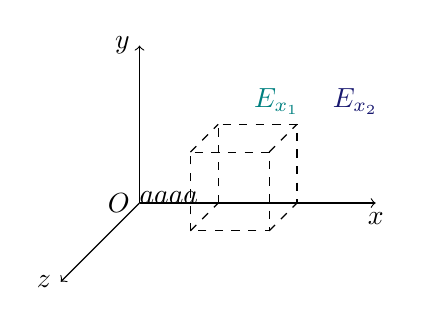
\begin{tikzpicture}
            \draw [->] (0,0) node [left] {$O$} -- (0,2) node [left] {$y$};
            \draw [->] (0,0) -- (3,0) node [below] {$x$};
            \draw [->] (0,0) -- (-1,-1) node [left] {$z$};
            \draw [dashed] (1,0) rectangle (2,1);
            \draw [dashed,xshift=-.25*sqrt(2)*1cm,yshift=-.25*sqrt(2)*1cm] (1,0) rectangle (2,1);
            \draw [dashed] ({1-.25*sqrt(2)},{1-.25*sqrt(2)}) -- (1,1) ({2-.25*sqrt(2)},{1-.25*sqrt(2)}) -- (2,1);
            \draw [dashed] ({1-.25*sqrt(2)},{-.25*sqrt(2)}) -- (1,0) ({2-.25*sqrt(2)},{-.25*sqrt(2)}) -- (2,0);
            \length{({-.25*sqrt(2)},{-.5*sqrt(2)})}{({1-.25*sqrt(2)},{-.5*sqrt(2)})}{$a$}{(.5,0)};
            \length{({1-.25*sqrt(2)},{-.5*sqrt(2)})}{({2-.25*sqrt(2)},{-.5*sqrt(2)})}{$a$}{(.5,0)};
            \length{({2.25-.25*sqrt(2)},{-.25-.25*sqrt(2)})}{(2.25,-.25)}{$a$}{({.5*sqrt(2)},{.5*sqrt(2)})};
            \length{(2.4,0)}{(2.4,1)}{$a$}{(0,.5)};
            \node [teal,anchor=south] at (1,1) {$\bm E_{x_1}$};
            \node [MidnightBlue,anchor=south] at (2,1) {$\bm E_{x_2}$};
        \end{tikzpicture}\vspace*{\fill}
    \end{problem}
\end{paracol}
\solute6
\begin{solution}
    高斯面的上、下、前、后表面电通量均为零，左表面电通量为$E_{x_1}S$，右表面的电通量为$E_{x_2}a^2$.
    由高斯定理$(E_{x_2}-E_{x_1})a^2=(ba-2ba)a^2=Q/\epsilon_0$得$Q=\epsilon ba^3=\qty{7.08e-11}\C$.
\end{solution}

\begin{problem} % {冲量与动量定理}
    水力采煤是用高压水枪喷出的强力水柱冲击煤层. 设水柱直径$D=\qty{30}\mm$，水速$v=\qty{56}{\m/\s}$，水的密度为$\rho=\qty{e6}{\g/\m^3}$，水柱垂直射在煤层表面上，冲击煤层后的速度为零，求水柱的平均冲力.
\end{problem}
\solute6
\begin{solution}
    $\d t$时间内的冲击煤层上的水动量变化为$\d p=v\d m\xlongequal[S=\pi D^2/4]{\d m=\rho Sv\d t}\pi\rho v^2 D^2\d t/4$，由动量定理$\d p=F\d t$得$F=\pi\rho v^2 D^2/4=\qty{2216.71}\N$.
\end{solution}

\begin{problem}
\begin{paracol}{2}
    A $\qty{500.0}{\g}$ bird is flying horizontally at $\qty{2.25}{\m/\s}$, not paying much attention, when it suddenly flies into a stationary vertical bar, hitting it $\qty{25.0}{\cm}$ below the top. The bar is uniform, $\qty{0.750}{\m}$ long, has a mass of $\qty{1.50}{\kg}$, and is hinged at its base. After the collision the velocity of the bird is $0$.
    \switchcolumn\vspace*{\fill}\centering
    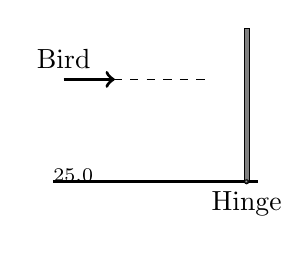
\begin{tikzpicture}[scale=.65]
        \draw [very thick] (0,0) -- (4,0);
        \draw [dashed] (.2,2) -- (3,2);
        \draw [very thick,->] (.2,2) -- (1.2,2) node [at start,above] {Bird};
        \length{(2,2)}{(2,3)}{$\scriptstyle\qty{25.0}\cm$}{(0,2)};
        \filldraw [fill=gray] (2.95,0) rectangle (3.05,3);
        \shade [ball color=black] (3,0) circle (0.05) node [below] {Hinge};
    \end{tikzpicture}\vspace*{\fill}
\end{paracol}
\begin{enumerate}
    \item What is the angular velocity of the bar just after it is hit by the bird?
    \item After the collision the bar tilts and falls on the ground. What is the angular velocity of the bar just as it reaches the ground?
\end{enumerate}
\end{problem}
\solute6
\begin{solution}\leavevmode
    \begin{enumerate}
        \item 由鸟和杆对杆下方支点角动量守恒$mv_0(l-h)=I\omega$得碰撞后杆的角速度$\omega=\qty2{\radian/\s}$.
        \item 杆子倒下过程中，由机械能守恒定律$I\omega^2/2+Mgl/2=I\omega'^2/2$得杆子刚接触地面时的角速度$\omega'=\sqrt{\omega^2+Mgl/I}=\qty{6.63}{\radian/\s}$. 其中$I=Ml^2/3$为杆绕底部的转动惯量.
    \end{enumerate}
\end{solution}

\begin{problem}
    双原子分子的原子作用力是保守力，表示成$\bm F=F_0\ab(r_0^6-r^6)\bm r/r^{12}$. 其中$r_0$为常数.
    \begin{enumerate}
        \item 设无穷远处为势能零点，试求出分子的势能函数$E_p(r)=\int_r^{\infty}{\bm F\cdot\d\bm r}$.
        \item 画出势能曲线简图.
        \item 计算分子势能为极小值时的原子间距.
    \end{enumerate}
\end{problem}
\begin{paracol}{2}
\solute6
\begin{solution}\leavevmode
    \begin{tasks}[label=\arabic*.](5)
        \task*(4) $E_p(r)=F_0(r_0^6/11r^{11}-1/5r^5)$.
        \task 见右图.
        \task! 分子势能极小时$\d E_p/\d r=F_0(-r_0^6/r^{12}+1/r^6)=0$，得此时原子间距$r=r_0$.
    \end{tasks}
    \switchcolumn\vspace*{\fill}\centering
    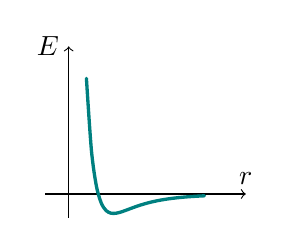
\begin{tikzpicture}[scale=1.5]
        \draw [->] (-.2,0) -- (1.5,0) node [above] {$r$};
        \draw [->] (0,-.2) -- (0,1.25) node [left] {$E$};
        \makeatletter
        \ifdefstring{\LITE@answer}{hideanswer}{\relax}{
            \draw [very thick,teal,variable=\x,domain=.15:1.15,smooth,line cap=round] plot ({\x},{.75*(1-(\x+0.75)^(5))/((\x+0.75)^(11))});
        }
        \makeatother
    \end{tikzpicture}\vspace*{\fill}
\end{solution}
\end{paracol}

\section{Calculate Premium (30 points in all)}

\begin{paracol}{2}
\begin{problem} % {电场强度}
    A semicircular ring of radius $R$ is centered at the origin in the $yz$-plane for $z\geq 0$. Charge $q$ is uniformly distributed around it.
\begin{enumerate}
    \item According to the symmetry, which component of the electric field is zero, $E_x$, $E_y$ or $E_z$?
    \item Find the electric field at a point $P$ on the ring axis at a distance $x$ from its center.
\end{enumerate}
\end{problem}
\switchcolumn\vspace*{\fill}\centering
\vfill
\begin{tikzpicture}[scale=1.5]
    \draw [->] (0,0) -- (0,2) node [left] {$y$};
    \draw [->] (0,0) -- (2,0) node [near end,below] {$P$} node [above] {$x$};
    \draw [->] (0,0) -- ({-.5*sqrt(2)},{-.5*sqrt(2)}) node [left] {$z$};
    \shade [ball color=MidnightBlue!50] (1.5,0) circle (0.05);
    \draw [very thick] (0,1) arc (90:270:.25 and 1);
\end{tikzpicture}\vspace*{\fill}
\vfill
\end{paracol}
\solute{20}
\begin{solution}
    \begin{enumerate}
        \item 由对称性易知$E_y=0$.
        \item 如图所示，作圆环上任一线元$\d l$到$O$点连线的反向延长线，与圆环顶端的切线相交于$A$，$B$两点. 由图中几何关系得，$AB=r'\d\theta/\sin\theta=R\d\theta/\sin^2{\theta}$.
        
        \begin{figure}[htbp]
            \centering
            \begin{tikzpicture}
                \draw [very thick,dashed] (-3,2) node [above] {$M$} -- (3,2) node (n) [above] {$N$};
                \draw [very thick] (-2.5,2) -- (2.5,2);
                \draw (-2,0) arc (180:0:2);
                \draw [->] (0,0) node [right] {$O$} -- (0,2) node [right,midway] {$R$};
                \draw [very thick,teal] (-2.5,2) node [above,black] {$\scriptstyle A$} -- (-2,2) coordinate (b) node [above,black] {$\scriptstyle B$} -- (0,0) -- cycle;
                \filldraw (0,0) coordinate (o) circle (.05);
                \pic["$\theta$", draw=DarkRed,very thick,angle eccentricity=1.5,angle radius=12]{angle=o--b--n};
                \draw [dotted] (b) -- ({-10*sqrt(82)/41},{8*sqrt(82)/41}) coordinate (d) node [below left] {$\scriptstyle D$};
                \draw [decorate,decoration={brace,raise=2pt}] (o) -- (d) node [midway,below left] {$r'$};
            \end{tikzpicture}
        \end{figure}
        而圆环上线元在$O$点产生的场强大小为$\d E=\lambda\d\theta/4\pi\epsilon_0R$.
        若顶端的切线均匀带电，电荷线密度为$\lambda'$，则$AB$在$O$点产生的场强大小为
        \[\d E'=\frac{1}{4\pi\epsilon_0}\frac{\lambda'AB}{r'^2}=\frac{1}{4\pi\epsilon_0}\frac{\lambda'R\d\theta/\sin^2{\theta}}{(R/\sin\theta)^2}
        =\frac{1}{4\pi\epsilon_0}\frac{\lambda'\d\theta}{R}\]
        若$\lambda'=\lambda$，则$\d E'=\d E$. 意味着均匀带电半圆环可由带有等量电荷线密度的无限长直线替代. 由高斯定理，无限长直带电线在P点的场强大小为$E=\lambda/2\pi\epsilon_0r=q/2\pi^2R\epsilon_0\sqrt{R^2+x^2}$.
    \end{enumerate}
\end{solution}

\begin{problem} % {牛顿运动定律，转动定律}
\begin{paracol}{2}
    A block of mass $m_A$ is dragging up along a frictionless surface inclined by an angle $\phi$ to the horizontal, a light cord (parallels to the slop) attached to it is wrapped around the shaft of a wheel mounted on the top of the incline. A block of mass $m_B$ is attached to the rim of the wheel by another light cord as shown in the figure below. Suppose the moment of inertia of the wheel is $I$, the radius of the wheel is $R$ and the radius of its shaft is $r$.
\switchcolumn\vspace*{\fill}\centering
\begin{tikzpicture}
    \filldraw [fill=MidnightBlue,fill opacity=.2] (0,0) coordinate (b) -- ({2*sqrt(3)},0) coordinate (a) --++ (0,2) coordinate (c) -- cycle;
    \pic["$\phi$",very thick,draw=DarkRed,angle eccentricity=1.35,angle radius=24]{angle=a--b--c};
    \draw ({2*sqrt(3)},2) circle (.3) circle (.6);
    \draw ({1.35+.3*sqrt(3)},{.65*sqrt(3)+.3}) -- ({2*sqrt(3)-.15},{2+.15*sqrt(3)});
    \draw [rotate around={30:(0,0)},xshift=sqrt(3)*1cm] (0,0) rectangle (.6,.6) node [midway,rotate=30] {$m_A$};
    \draw ({2*sqrt(3)+.6},2) --++ (0,-1);
    \draw ({2*sqrt(3)+.3},1) rectangle ({2*sqrt(3)+.9},.4) node [midway] {$m_B$};
    \ifdefstring{\LITE@answer}{ans}{
        \draw [<->,very thick,MidnightBlue,opacity=.6] ({2*sqrt(3)+.6},-.3) --++ (0,1.8);
        \draw [->,very thick,MidnightBlue,opacity=.6] ({1.35+.15*sqrt(3)},{.65*sqrt(3)+.15}) -- ++ (0,-1);
        \draw [->,very thick,MidnightBlue,opacity=.6] ({1.35+.15*sqrt(3)},{.65*sqrt(3)+.15}) -- ++ ({-.25*sqrt(3)},{.75});
        \draw [->,very thick,MidnightBlue,opacity=.6] ({1.35+.15*sqrt(3)},{.65*sqrt(3)+.15}) -- ++ ({.375*sqrt(3)},{.375});
    }{\relax}
\end{tikzpicture}\vspace*{\fill}
\end{paracol}
\begin{tasks}[label=\arabic*.](2)
    \task* Draw the free-body force diagrams for the wheel and the blocks.
    \task Find the angular acceleration of the wheel.
    \task Find the acceleration of the two blocks.
\end{tasks}
\end{problem}
\solute{20}
\begin{solution}\leavevmode
    受力分析如图所示. 分别对两物块列牛顿运动定律，对轮子列转动定律得
    \[\begin{dcases}
            m_Ag-T_A=m_Aa_A\\
            T_B-m_Bg\sin\phi=m_Ba_B\\
            T_AR-T_Br=I\beta
    \end{dcases}\]
    代入关系$a_i=r_i\beta$得轮子的角加速度和两物块的加速度分别为
    \[\beta=\frac{m_AgR-m_Bgr\sin\phi}{I+m_AR^2+m_Br^2},\ a_A=\frac{m_AgR^2-m_BgRr\sin\phi}{I+m_AR^2+m_Br^2},\ a_B=\frac{m_AgRr-m_Bgr^2\sin\phi}{I+m_AR^2+m_Br^2}\]
\end{solution}